\chapter{Waveform Groups}

A waveform group is a collection of one or more waveforms stacked vertically under a common timeline. All waveforms
within a group share the same timeline and vertical cursor(s).

When glscopeclient starts up, by default all channels on the attached instruments are displayed in a single waveform
group (Figure \ref{single-group}).

\begin{figure}[h]
\centering
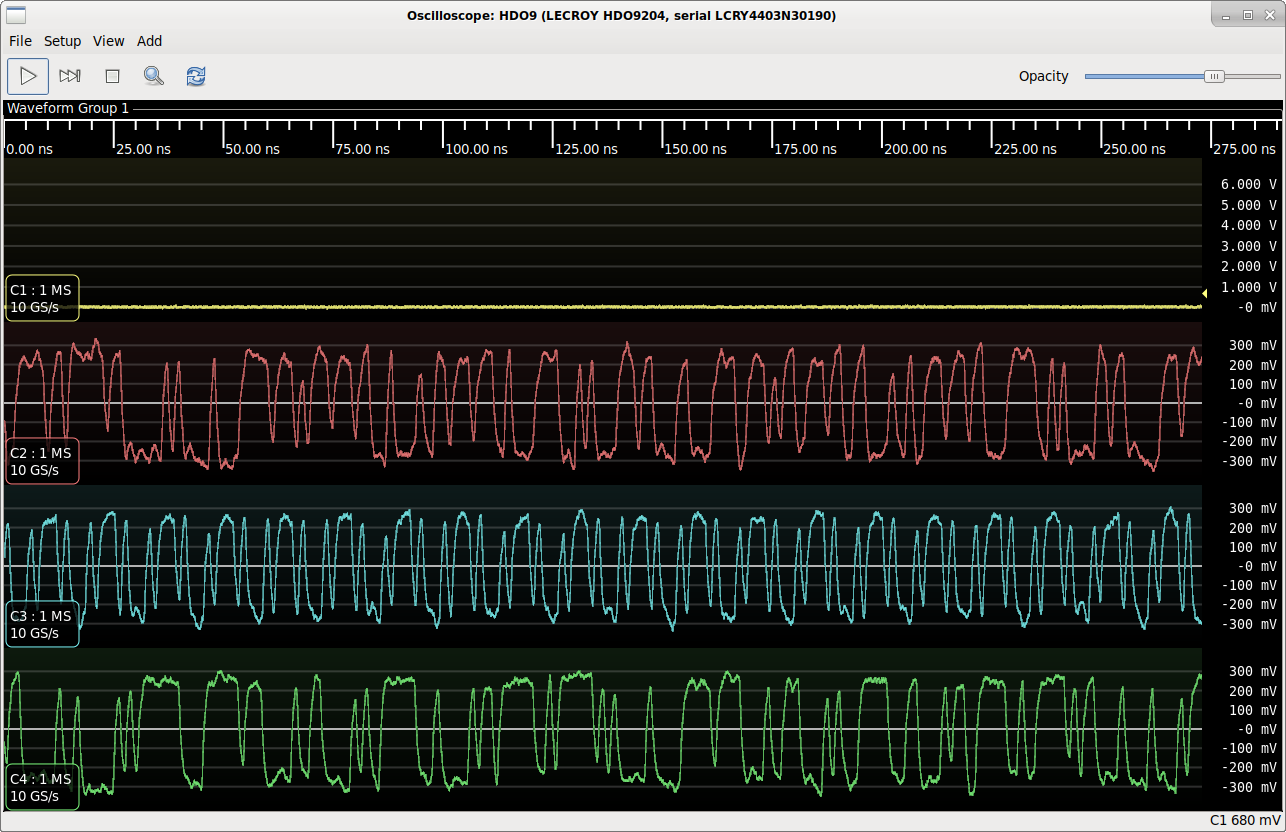
\includegraphics[width=13cm]{images/overview.png}
\caption{Top level glscopeclient window with a single waveform group}
\label{single-group}
\end{figure}

As you add protocol decodes or look at different parts of a waveform, it may be helpful to create additional waveform
groups. Typical reasons for creating additional groups include:

\begin{itemize}
\item Zooming into one set of signals to see detail on short time scales while maintaining a high level overview of
others
\item Viewing signals with incompatible horizontal units. For example, a FFT has horizontal units of frequency while an
analog waveform has horizontal units of time. Eye patterns also have horizontal units of time, but are always displayed
as two UIs wide and cannot be zoomed.
\end{itemize}

\section{Managing Groups}

Additional groups may be created by right clicking a waveform and selecting \menustyle{[Move|Copy] waveform to / Insert
new group at [right|bottom]} from the context menu. This will split the current group's area in half horizontally or
vertically, with the selected waveform moved or copied to the newly added group and all other waveforms in the original
group.

Waveforms may be also be moved within, or between, groups by clicking the channel information box and dragging it. A
yellow insertion bar will appear when dragging, showing the location the waveform will be inserted in.

If a waveform is dragged to the very bottom or right side of a waveform group, the destination group will be split
vertically or horizontally and the new waveform will be inserted below or to the right of the destination group. The
insertion bar turns orange when dragging near the edge of a group, to indicate that a split will take place.

Dividers between waveform groups may be dragged with the left mouse button. Any group may be subdivided again, to
create arbitrarily complex tiles of waveforms. Figure \ref{multiple-groups} shows a two-level hierarchy created by
moving channel 2 to a new group at right, then moving channel 4 to a new group below that one.

\begin{figure}[h]
\centering
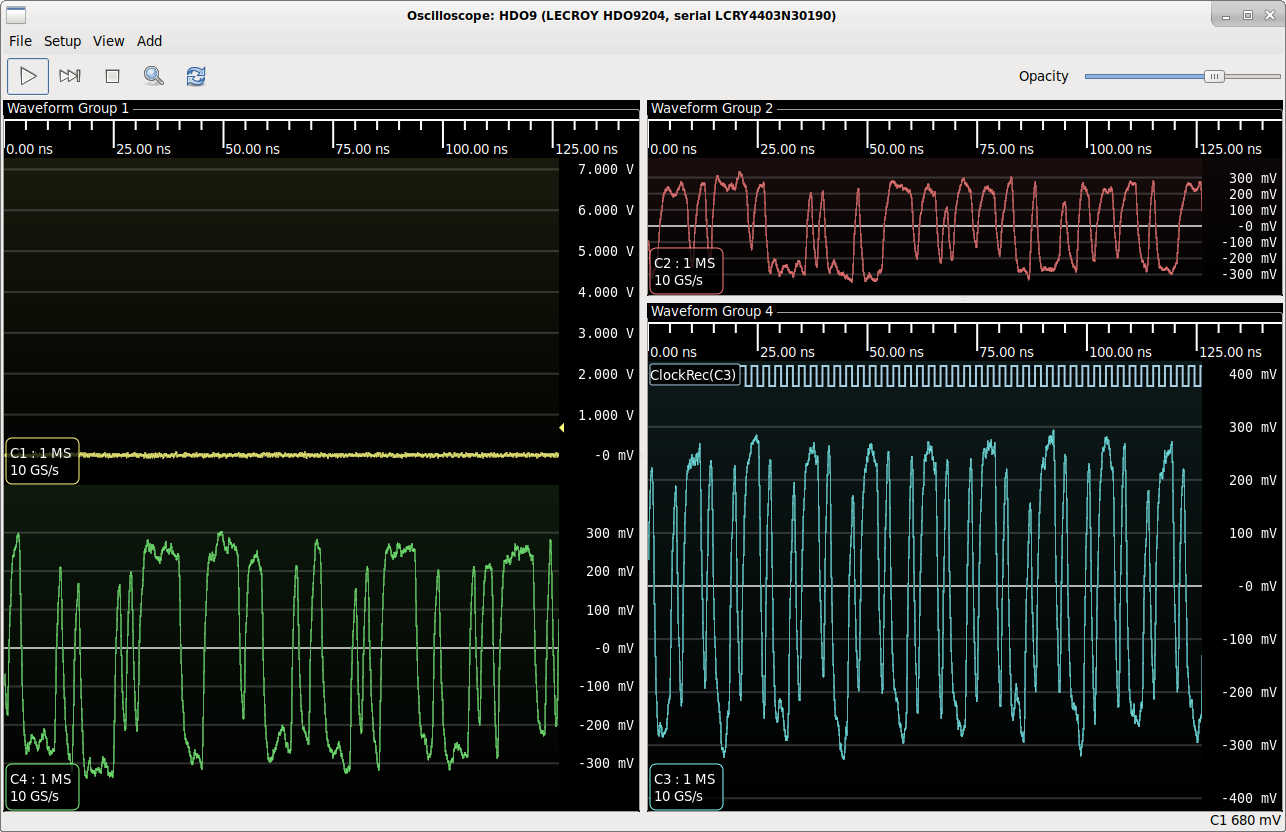
\includegraphics[width=14cm]{images/multiple-groups.png}
\caption{Top level glscopeclient window with several waveform groups separated by splitters}
\label{multiple-groups}
\end{figure}

Protocol decode overlays may be reordered by dragging the channel information box with the mouse, however they cannot
currently be moved to another waveform or group.

New waveform groups are given an automatically generated name when created, for example "Waveform Group 2". This name
will be editable in a future software release (scopehal-apps:53).
